\documentclass{article}
\usepackage[top=3cm, bottom=3cm, left = 2cm, right = 2cm]{geometry} 
\geometry{a4paper} 
\usepackage[T1]{polski}
\usepackage[utf8]{inputenc}
\usepackage{titling}
\usepackage{caption}
\usepackage{algorithm}
\usepackage{algpseudocode}
\usepackage[parfill]{parskip}
\usepackage{multirow}
\usepackage{graphicx}
\usepackage{amsmath}


\renewcommand\maketitlehooka{\null\mbox{}\vfill}
\renewcommand\maketitlehookd{\vfill\null}

\floatname{algorithm}{Algorytm}
\algrenewcommand\algorithmicrequire{\textbf{Input:}}
\algrenewcommand\algorithmicensure{\textbf{Output:}}

\newcommand*\Heq{\ensuremath{\overset{\kern2pt H}{=}}}

\title{Obliczenia Naukowe}
\author{Karol Janic}
\date{3 listopada 2023}

\begin{document}

\begin{titlingpage}
    \maketitle
\end{titlingpage}

\tableofcontents

\newpage

\section{Zadanie 1}
\subsection{Cel}
Celem zadania jest zbadanie wpływu niewielkich zmian w danych na wyniki obliczania iloczynu skalarnego czterami metodami:
\begin{itemize}
    \item "w przód"
    \item "w tył"
    \item "od największego do najmniejszego"
    \item "od najmniejszego do największego"
\end{itemize} 

\subsection{Rozwiązanie}
Zaimplementowano cztery algorytmy(opisane na poprzedniej liście) oraz porównano ich działanie 
\newline dla różnych arytmetyk zmiennopozycyjnych: \texttt{Float32}, \texttt{Float64} i dwóch par wektorów: $\left< X, Y \right>$, $\left< X', Y \right>$, \newline gdzie:
\begin{itemize}
    \item $X = [2.718281828, -3.141592654, 1.414213562, 0.5772156649, 0.3010299957]$ 
    \item $X' = [2.718281828, -3.141592654, 1.414213562, 0.577215664, 0.301029995]$
    \item $Y = [1486.2497, 878366.9879, -22.37492, 4773714.647, 0.000185049]$ 
\end{itemize}

\subsection{Wyniki i wnioski}
\begin{table}[h!]
    \centering
    \begin{tabular}{|c|c|c|c|c|}
    \hline 
    \multirow{3}{*}{metoda} & \multicolumn{4}{|c|}{typ} \\ 
    \cline{2-5}
    & \multicolumn{2}{|c|}{\texttt{Float32}} & \multicolumn{2}{|c|}{\texttt{Float64}}  \\ 
    \cline{2-5}
    & $\left< X, Y \right>$ & $\left< X', Y \right>$ & $\left< X, Y \right>$ & $\left< X', Y \right>$ \\
    \hline
    "w przód" & -0.4999443 & -0.4999443 & 1.0251881368296672e-10 & -0.004296342739891585 \\
    \hline 
    "w tył" & -0.454345 & -0.454345 & -1.5643308870494366e-10 & -0.004296342998713953 \\
    \hline 
    "od największego ..." & -0.5  & -0.5 & 0.0 & -0.004296342842280865 \\
    \hline 
    "od najmniejszego ..." & -0.5  & -0.5 & 0.0 & -0.004296342842280865 \\
    \hline
    \end{tabular}
    \caption{Porównanie wartości obliczonego iloczynu skalarnego.}
\end{table}

Modyfikacje danych nie wpłynęły na wynik obliczeń w pojedynczej precyzji, ponieważ zaszły one na miejscach poza precyją arytmetyki.
Cyfry zostały usunięte na $10$-tym miejscu po przecinku zaś precyzja arytmetyki w przybliżeniu wynosi $10^{-7}$.

W podwójnej precyzji wyniki po modyfikacji znacząco różnią się od wyników uzyskanych początkowo. Powodem dużej zmiany wartości wyniku przy małej zmianie wartości argumentów jest to, że zadanie jest źle uwarunkowane. Wskaźnikiem uwarunkowania tego zadanie jest:
$$
cond(X, Y) = \frac{\sum_{i=1}^{n} |X_iY_i|}{|\sum_{i=1}^{n} X_iY_i|}
$$
Łatwo zauważyć, że osiąga on dużą wartość, gdy wektory są prawie prostopadłe tak jak w przypadku wektorów danych w zadaniu.


\newpage

\section{Zadanie 2}
\subsection{Cel}
Celem zadania jest sprawdzenia jak programy do wizualizacji radzą sobie z funkcją $f(x)=e^x \ln (1+e^{-x})$.

\subsection{Rozwiązanie}
W celu oceny poprawności wizualizacji obliczono granice funkcji w $+\infty$:
$$
\lim_{x \rightarrow +\infty} e^x \cdot \ln(1 + e^{-x}) = \lim_{x \rightarrow +\infty} \frac{\ln(1 + e^{-x})}{e^{-x}} \Heq \lim_{x \rightarrow +\infty} \frac{-\frac{e^{-x}}{1 + e^{-x}}}{-e^{-x}} = \lim_{x \rightarrow +\infty} \frac{1}{1 + e^{-x}} = 1
$$
Następnie użyto \texttt{Pyplot}, \texttt{Plots.jl} oraz \texttt{Gnuplot.jl} do wizualizacji funkcji.

\subsection{Wyniki i wnioski}
Wizualizacje pokrywają się właściwymi wartościami funkcji dla wartości mniejszych niż $30$. Dla wartości pomiędzy $30$ a $36$ widoczne są oscylacje. Dla argumentów większych niż 37 wizualizacja prezentuje niezmiennie $0$.
Wszystkie 3 narzędzia do wizualizacji wprowadzają użytkownika w błąd. 
\newline Wartości $0$ dla argumentów większych od $37$ biorą się stąd, że w tym przypadku $e^x$ przyjmuje wartości mniejsze niż epsilon maszynowy dla arytmetyki z podwójną prezycją. Wówczas logarytm obliczany jest dla argumentu $1$, przyjmuje wartość $0$ i całe wyrażenia także ma wartość $0$.
\newline Powodem oscylacji jest mnożenie bardzo dużej liczby $e^x$ i bardzo małej liczby $\ln(1 + e^{-x})$. Skutkuje to utratą precyzji.

\begin{figure}[h!]
    \centering
    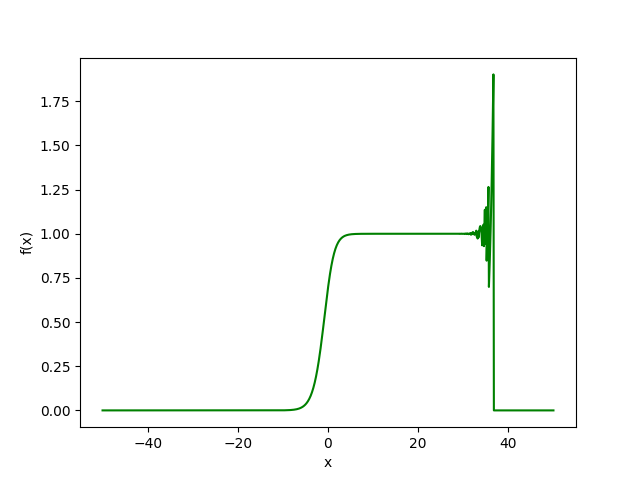
\includegraphics[scale=0.5]{plots/f(x)-1-pyplot.png}
    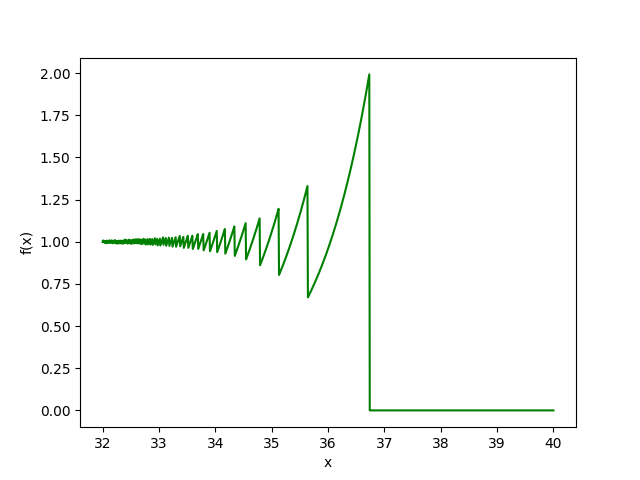
\includegraphics[scale=0.5]{plots/f(x)-2-pyplot.png}
    \caption{Wizualizacji za pomocą Pyplot}
\end{figure}

\begin{figure}[h!]
    \centering
    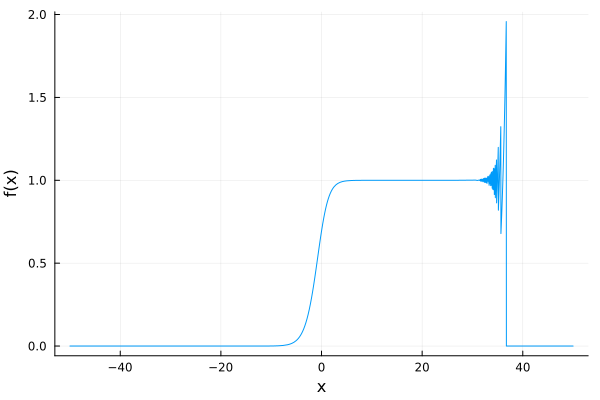
\includegraphics[scale=0.365]{plots/f(x)-1-plots.png}
    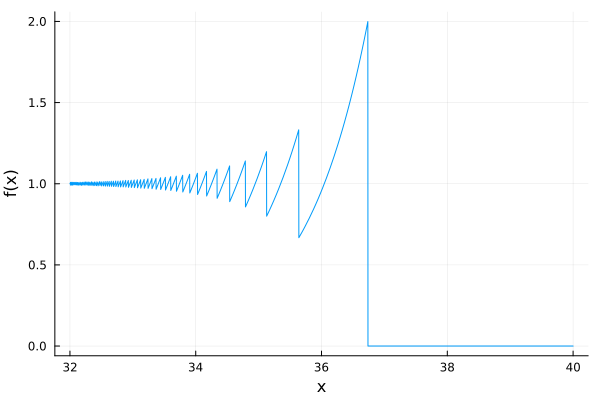
\includegraphics[scale=0.365]{plots/f(x)-2-plots.png}
    \caption{Wizualizacji za pomocą Plots.jl}
\end{figure}

\begin{figure}[h!]
    \centering
    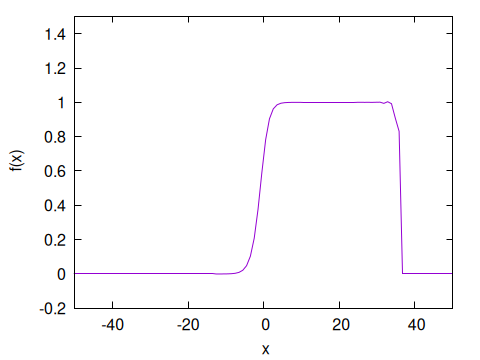
\includegraphics[scale=0.49]{plots/f(x)-1-gnuplot.png}
    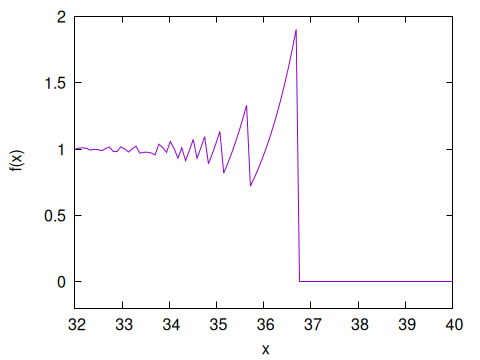
\includegraphics[scale=0.49]{plots/f(x)-2-gnuplot.png}
    \caption{Wizualizacji za pomocą Gnuplot.jl}
\end{figure}

\newpage

\section{Zadanie 3}
\subsection{Cel}
Celem zadania jest porównanie metod służących rozwiązywaniu układów równań liniowych $Ax = b$:
\begin{itemize}
    \item metoda eliminacji Gaussa
    \item metoda korzystająca z odwrotności macierzy
\end{itemize}
na macierzach:
\begin{itemize}
    \item Hilberta $A = H_n$ dla $n > 1$
    \item losowych $A = R_n$ dla $n=5, 10, 20$ z rosnącym wskaźnikiem uwarunkowania $c = 1, 10, 10^3, 10^7, 10^{12}, 10^{16}$
\end{itemize}

\subsection{Rozwiązanie}
Przy użyciu dostarczonych funkcji wygenerowano odpowiednie macierze $A$. Następnie przy użyciu zaimplementowanych metod rozwiązano te układy równań, obliczono błędy względne i je porównano.

\newpage
\subsection{Wyniki i wnioski}
W poniższych tabelach przedstawiono otrzymane wyniki. $\delta_{GAUSS}$, $\delta_{INV}$ oznaczają błędy względne wektora wyznaczonego metodą Gaussa oraz metodą bazującą na macierzy odwrotnej względem wektora oczekiwanego.
\newline Wartości wskaźników uwarunkowania dla macierzy Hilberta szybko rosną. Gdy $n$ osiąga wartość $13$ błąd obu metod przekracza $100\%$ dokładnej wartości. Metoda eliminacji Gaussa zwraca wektory bliższe dokładnemu, jednak nie jest to znacząca różnica.
\newline W przypadku macierzy losowych ich wielkość nie wpływa na błąd względny. Zależy on jedynie od wskaźnika uwarunkowania macierzy. W tym przypadku metoda Gaussa także zwraca trochę dokładniejsze wyniki. Błąd względny przekracza $100\%$ dla wskaźnikiem uwarunkowania macierzy rzędu $10^{16}$.
\newline Problem rozwiązania układu równań $Ax = b$, gdzie $A$ jest macierzą Hilberta lub losową macierzą o dużej wartości wskaźnika uwarunkowania jest problemem źle uwarunkowanym. Błędy względne zależą od wartości wskaźnika uwarunkowania zadania.  Z powyższych obserwacji można wysnuć wniosek, że błąd względny jest równy w przybliżeniu iloczynowy epsilona maszynowego dla danej arytmetyki z wartością wskaźnika uwarunkowania macierzy.
\begin{table}[h!]
    \centering
    \begin{tabular}{ |c|c|c|c|c| } 
        \hline 
        $n$ & $rank(H_n)$ & $cond(H_n)$ & $\delta_{GAUSS}$ & $\delta_{INV}$ \\
        \hline
        2 & 2 & 1.93e+01 & 5.66e-16 & 1.12e-15 \\ 
        \hline
        3 & 3 & 5.24e+02 & 8.35e-15 & 9.83e-15 \\ 
        \hline
        4 & 4 & 1.55e+04 & 4.23e-13 & 3.96e-13 \\ 
        \hline
        5 & 5 & 4.77e+05 & 1.26e-12 & 8.13e-12 \\ 
        \hline
        6 & 6 & 1.50e+07 & 1.54e-10 & 1.04e-10 \\ 
        \hline
        7 & 7 & 4.75e+08 & 6.52e-09 & 4.33e-09 \\ 
        \hline
        8 & 8 & 1.53e+10 & 3.60e-07 & 4.02e-07 \\ 
        \hline
        9 & 9 & 4.93e+11 & 1.32e-05 & 1.46e-05 \\ 
        \hline
        10 & 10 & 1.60e+13 & 4.19e-04 & 4.07e-04 \\ 
        \hline
        11 & 10 & 5.22e+14 & 1.00e-02 & 1.06e-02 \\ 
        \hline
        12 & 11 & 1.64e+16 & 5.50e-01 & 6.70e-01 \\ 
        \hline
        13 & 11 & 4.49e+18 & 7.02e+01 & 8.27e+01 \\ 
        \hline
        14 & 11 & 3.22e+17 & 9.65e+00 & 1.01e+01 \\ 
        \hline
        15 & 12 & 3.37e+17 & 6.92e+02 & 7.16e+02 \\ 
        \hline
    \end{tabular}
    \caption{Porównanie błędów względnych rozwiązań układów równań, gdy $A = H_n$.}
\end{table}

\begin{table}[h!]
    \centering
    \begin{tabular}{ |c|c|c|c|c|c|c|c|c|c| } 
        \hline
         & \multicolumn{3}{|c|}{$n = 5$} & \multicolumn{3}{|c|}{$n = 10$} & \multicolumn{3}{|c|}{$n = 15$} \\
        \cline{2-10}
        $c$ & $rank(R_n)$ & $\delta_{GAUSS}$ & $\delta_{INV}$ & $rank(R_n)$ & $\delta_{GAUSS}$ & $\delta_{INV}$ & $rank(R_n)$ & $\delta_{GAUSS}$ & $\delta_{INV}$ \\
        \hline
        1 & 5 & 1.72e-16 & 2.28e-16 & 10 & 2.28e-16 & 2.25e-16 & 20 & 3.99e-16 & 3.58e-16 \\ 
        \hline
        10 & 5 & 1.99e-16 & 1.40e-16 & 10 & 3.22e-16 & 2.65e-16 & 20 & 4.45e-16 & 3.86e-16 \\ 
        \hline
        $10^3$ & 5 & 3.06e-14 & 2.89e-14 & 10 & 1.40e-14 & 1.27e-14 & 20 & 6.82e-14 & 6.75e-14 \\ 
        \hline
        $10^7$ & 5 & 2.50e-10 & 3.09e-10 & 10 & 7.24e-12 & 1.78e-11 & 20 & 1.35e-10 & 7.81e-11 \\ 
        \hline
        $10^{12}$ & 5 & 2.08e-05 & 8.73e-06 & 10 & 4.45e-06 & 5.46e-06 & 20 & 4.20e-05 & 4.13e-05 \\ 
        \hline
        $10^{16}$ & 4 & 1.59e-01 & 1.51e-01 & 9 & 2.68e-01 & 2.69e-01 & 19 & 7.00e-02 & 1.08e-01 \\ 
        \hline
    \end{tabular}
    \caption{Porównanie błędów względnych rozwiązań układów równań, gdy $A = R_n$ oraz $c$ jest wskaźnikiem uwarunkowania macierzy $A$.}
\end{table}

\newpage

\section{Zadanie 4}
\subsection{Cel}
Celem zadania jest zbadanie pierwiastków "złośliwego wielomianu" Wilkinsona dla wersji z niezaburzonymi współczynnikami oraz wersji z zaburzonym jednym ze współczynników. Wersja z niezaburzonymi współczynnikami:
\begin{center}
    $p(x) = (x-20)(x-19)(x-18)(x-17)(x-16)(x-15)(x-14)(x-13)(x-12)(x-11)(x-10)\newline(x-9)(x-8)(x-7)(x-6)(x-5)(x-4)(x-3)(x-2)(x-1)$
\end{center}

\subsection{Rozwiązanie}
Przy użyciu funkcji \texttt{roots} pakietu \texttt{Polynomials} obliczono pierwiastki wielomianu $p(x)$ w postaci naturalnej $P(x)$. Następnię zaburzono współczynnik przy $x^{19}$ z $210$ na $210 - 2^{-23}$ i raz jeszcze obliczono pierwiastki wielomianu $p'(x)$. Następnie porównano je z wartościami dokładnymi.

\subsection{Wyniki i wnioski}
\begin{table}[h!]
    \centering
    \begin{tabular}{ |c|c|c|c|c| }
    \hline
    $k$ & $z_k$ & $|P(z_k)|$ & $|p(z_k)|$ & $|z_k - k|$ \\ 
    \hline
    1 & 1.000000 & 35696.509648 & 36626.425482 & 0.000000 \\ 
    \hline
    2 & 2.000000 & 176252.600267 & 181303.933673 & 0.000000 \\ 
    \hline
    3 & 3.000000 & 279157.696882 & 290172.285889 & 0.000000 \\ 
    \hline
    4 & 4.000000 & 3027109.298899 & 2041537.290275 & 0.000000 \\ 
    \hline
    5 & 5.000001 & 22917473.756567 & 20894625.006962 & 0.000001 \\ 
    \hline
    6 & 5.999989 & 129024172.842051 & 112504845.775630 & 0.000011 \\ 
    \hline
    7 & 7.000102 & 480511275.460206 & 457290864.273095 & 0.000102 \\ 
    \hline
    8 & 7.999356 & 1637952021.896114 & 1555645937.735738 & 0.000644 \\ 
    \hline
    9 & 9.002915 & 4877071372.550003 & 4687816175.648389 & 0.002915 \\ 
    \hline
    10 & 9.990413 & 13638638195.458128 & 12634601896.949205 & 0.009587 \\ 
    \hline
    11 & 11.025023 & 35856312951.308647 & 33001284744.984150 & 0.025023 \\ 
    \hline
    12 & 11.953283 & 75333323603.581970 & 73885256654.049881 & 0.046717 \\ 
    \hline
    13 & 13.074314 & 196059881243.308167 & 184762150931.441925 & 0.074314 \\ 
    \hline
    14 & 13.914756 & 357513478231.043152 & 355142775284.208435 & 0.085244 \\ 
    \hline
    15 & 15.075494 & 821627123645.597046 & 842320155896.425415 & 0.075494 \\ 
    \hline
    16 & 15.946287 & 1551497888049.406738 & 1570728736625.802002 & 0.053713 \\ 
    \hline
    17 & 17.025427 & 3694735918486.229004 & 3316978223889.236328 & 0.025427 \\ 
    \hline
    18 & 17.990921 & 7650109016515.867188 & 6344853141791.280273 & 0.009079 \\ 
    \hline
    19 & 19.001910 & 11435273749721.195312 & 12285717366719.660156 & 0.001910 \\ 
    \hline
    20 & 19.999809 & 27924106393680.726562 & 23183095352716.378906 & 0.000191 \\ 
    \hline
    \end{tabular}
    \caption{Rzeczywiste pierwiastki dla niezaburzonego wielomianu}
\end{table}

\begin{table}[h!]
    \centering
    \begin{tabular}{ |c|c|c|c|c| }
    \hline
    $k$ & $z_k$ & $|P'(z_k)|$ & $|p'(z_k)|$ & $|z_k - k|$ \\ 
    \hline
    1 & 1.000000 & 20259.872313 & 19987.872313 & 0.000000 \\ 
    \hline
    2 & 2.000000 & 346541.413759 & 352369.413809 & 0.000000 \\ 
    \hline
    3 & 3.000000 & 2258059.700120 & 2416241.558252 & 0.000000 \\ 
    \hline
    4 & 4.000000 & 10542631.790395 & 11263702.300292 & 0.000000 \\ 
    \hline
    5 & 4.999999 & 37578309.165852 & 44757444.238069 & 0.000001 \\ 
    \hline
    6 & 6.000020 & 131409433.255694 & 214210316.580393 & 0.000020 \\ 
    \hline
    7 & 6.999602 & 393935587.464762 & 1784617342.786064 & 0.000398 \\ 
    \hline
    8 & 8.007772 & 1184986961.371896 & 18686972170.009857 & 0.007772 \\ 
    \hline
    9 & 8.915816 & 2225522123.307771 & 137463097751.429932 & 0.084184 \\ 
    \hline
    10 & - & - & - & - \\ 
    \hline
    11 & - & - & - & - \\ 
    \hline
    \vdots & \vdots & \vdots & \vdots & \vdots \\
    \hline
    18 & - & - & - & - \\ 
    \hline
    19 & - & - & - & - \\ 
    \hline
    20 & 20.846910 & 8756386551865.696289 & 1374374355999759872.000000 & 0.846910 \\ 
    \hline
    \end{tabular}
    \caption{Rzeczywiste pierwiastki dla zaburzonego wielomianu}
\end{table}

\newpage

Dokładność wartości wyznaczanych pierwiastków niezaburzonego wielomianu spada wraz z ich rosnącym indeksem. Pierwsze pierwiastki wyznaczane są z zadowalającą dokładnością, zaś blędy względne ponad połowy pierwiastków są rzędu kilku procent.
Wartości wielomianu w jego pierwiastkach okazują się całkowicie niezgodne z przewidywaniami niezależnie od użytej reprezentacji wielomianu. Powodem takich niedokładności jest niewystarczająca liczba cyfr znaczących reprezentacji w arytmetyce podwójnej precyzji($15-17$ cyfr znaczących) - wyznaczanie wartości wielomianu Wilkinsona w punkcie wymaga mnożeń liczb, które mają więcej cyfr znaczących. Nawet jeżeli jeden z czynników jest bliski wartości $0$ to kolejne niedokładne mnożenia powodują otrzymanie dużej liczby.
\newline W przypadku wielomianu zaburzonego dokładność wyznaczonych pierwiastków rzeczywistych jest mniejsza niż w przypadku wielomianu niezaburzonego. Dodatkowo tylko połowa pierwiastków została znaleziona. Metoda $roots$ zwróciła $10$ pierwiastków będących liczbami zepolonymi. Przyczyną takich wyników jest złe uwarunkowanie zadania. Zaburzenie jednego ze współczynników wielomianu Wilkinsona o $\epsilon$ na $19$ pozycji powoduje zaburzenia pierwiastka $x_{19} = 19$ o $-\epsilon \frac{19^{19}}{18!} \approx -\epsilon 10^{8}$ co dla $\epsilon = 2^{-23}$ daje około $30$.

\section{Zadanie 5}
\subsection{Cel}
Celem zadania jest przeprowadzenie symulacji modelu logistycznego, który jest opisany poprzez zależność:
$$p_{n+1} = p_n + r \cdot p_n(1 - p_n), \qquad n = 0, 1, 2, ...$$

\subsection{Rozwiązanie}
Przeprowadzono 40 iteracji eksperymentu dla $p_0 = 0.01$ oraz $r=3$ w dwóch wariantach w arytmetyce \texttt{Float32}. W pierwszym wyniki pośrednie nie były modyfikowane, zaś w drugim wynik pośredni $p_{10}$ został zaokrąglony do 3 miejsc po przecinku.
Dodatkowo powtórzono pierwszy wariant w arytmetyce \texttt{Float64}.

\subsection{Wyniki i wnioski}
Wyniki przeprowadzonej symulacji porównane zostały w tabeli. Łatwo zauważyć, że zarówno względnie małe zaburzenie czy zmiana prezycji arytmetyki ma bardzo duży wpływ na przebieg symulacji, ponieważ na przestrzeni kilkudziesięciu iteracji widać, że wyniki różnią się diametralnie.
\newline Powodem takich rozbieżności jest zbyt mała liczba cyfr w rozwinięciu liczby. Produkt dwóch liczb o $k_1$ i $k_2$ bitach potrzebnych na zapisanie części ułamkowej potrzebuje zazwyczaj $k_1 + k_2$ bitów na zapisanie części ułamkowej. Ponieważ wyznaczenie każdej kolejnej wartości $p_n$ wymaga mnożenia to bardzo szybko dostępna liczba bitów jest niewystarczająca. Już w $5$ iteracji wartości wyznaczane w arytmetyce o podwójnej precyzji różnią sie od tych liczonych w arytmetyce o pojedynczej precyzji na $6$ miejscu po przecinku. Wynika z tego, że właśnie w tym momencie obliczenia $p_n$ we \texttt{Float32} stają się niedokładne i błąd zaczyna sie kumulować. 

\begin{table}[h!]
    \centering
    \begin{tabular}{ |c|c|c|c| }
    \hline
    $n$ & niezaburzone $p_n$ w \texttt{Float32} & zaburzone $p_n$ w \texttt{Float32} & niezaburzone $p_n$ w \texttt{Float64} \\
    \hline
    1 & 0.0397 & 0.0397 & 0.0397 \\
    \hline
    2 & 0.15407173 & 0.15407173 & 0.15407173000000002 \\
    \hline
    3 & 0.5450726 & 0.5450726 & 0.5450726260444213 \\
    \hline
    4 & 1.2889781 & 1.2889781 & 1.2889780011888006 \\
    \hline
    5 & 0.1715188 & 0.1715188 & 0.17151914210917552 \\
    \hline
    6 & 0.5978191 & 0.5978191 & 0.5978201201070994 \\
    \hline
    7 & 1.3191134 & 1.3191134 & 1.3191137924137974 \\
    \hline
    8 & 0.056273222 & 0.056273222 & 0.056271577646256565 \\
    \hline
    9 & 0.21559286 & 0.21559286 & 0.21558683923263022 \\
    \hline
    10 & 0.7229306 & 0.722 & 0.722914301179573 \\
    \hline
    11 & 1.3238364 & 1.3241479 & 1.3238419441684408 \\
    \hline
    12 & 0.037716985 & 0.036488414 & 0.03769529725473175 \\
    \hline
    13 & 0.14660022 & 0.14195944 & 0.14651838271355924 \\
    \hline
    14 & 0.521926 & 0.50738037 & 0.521670621435246 \\
    \hline
    15 & 1.2704837 & 1.2572169 & 1.2702617739350768 \\
    \hline
    16 & 0.2395482 & 0.28708452 & 0.24035217277824272 \\
    \hline
    17 & 0.7860428 & 0.9010855 & 0.7881011902353041 \\
    \hline
    18 & 1.2905813 & 1.1684768 & 1.2890943027903075 \\
    \hline
    19 & 0.16552472 & 0.577893 & 0.17108484670194324 \\
    \hline
    20 & 0.5799036 & 1.3096911 & 0.5965293124946907 \\
    \hline
    21 & 1.3107498 & 0.09289217 & 1.3185755879825978 \\
    \hline
    22 & 0.088804245 & 0.34568182 & 0.058377608259430724 \\
    \hline
    23 & 0.3315584 & 1.0242395 & 0.22328659759944824 \\
    \hline
    24 & 0.9964407 & 0.94975823 & 0.7435756763951792 \\
    \hline
    25 & 1.0070806 & 1.0929108 & 1.315588346001072 \\
    \hline
    26 & 0.9856885 & 0.7882812 & 0.07003529560277899 \\
    \hline
    27 & 1.0280086 & 1.2889631 & 0.26542635452061003 \\
    \hline
    28 & 0.9416294 & 0.17157483 & 0.8503519690601384 \\
    \hline
    29 & 1.1065198 & 0.59798557 & 1.2321124623871897 \\
    \hline
    30 & 0.7529209 & 1.3191822 & 0.37414648963928676 \\
    \hline
    31 & 1.3110139 & 0.05600393 & 1.0766291714289444 \\
    \hline
    32 & 0.0877831 & 0.21460639 & 0.8291255674004515 \\
    \hline
    33 & 0.3280148 & 0.7202578 & 1.2541546500504441 \\
    \hline
    34 & 0.9892781 & 1.3247173 & 0.29790694147232066 \\
    \hline
    35 & 1.021099 & 0.034241438 & 0.9253821285571046 \\
    \hline
    36 & 0.95646656 & 0.13344833 & 1.1325322626697856 \\
    \hline
    37 & 1.0813814 & 0.48036796 & 0.6822410727153098 \\
    \hline
    38 & 0.81736827 & 1.2292118 & 1.3326056469620293 \\
    \hline
    39 & 1.2652004 & 0.3839622 & 0.0029091569028512065 \\
    \hline
    40 & 0.25860548 & 1.093568 & 0.011611238029748606 \\
    \hline
    \end{tabular}
    \caption{Wyniki symulacji modelu logistycznego}
\end{table}

\newpage

\section{Zadanie 6}
\subsection{Cel}
Celem zadania jest przeprowadzenie eksperymentu, który polega na wyznaczaniu kolejnych wartości ciągu zdefiniowanego równaniem rekurencyjnym:
$$x_{n+1} = x_n^2 + c, \qquad n = 0, 1, 2, ...$$ 

\subsection{Rozwiązanie}
Punkty stałe:
\begin{enumerate}
    \item dla $c = -2$ punktami stałymi są $-1$ oraz $2$
    \item dla $c = -1$ punktami stałymi są $\frac{1 + \sqrt{5}}{2}$ oraz $\frac{1 - \sqrt{5}}{2}$
\end{enumerate}
Wyznaczono $40$ pierwszych elementów ciągu dla różnych konfiguracji $x_0$ oraz $c$. Następnie przeprowadzono iterację graficzną podanego równania rekurencyjnego.

\subsection{Wyniki i wnioski}
Wartości elementów ciągu kształtują się tak samo dla $x_0$ jak i dla $-x_0$. 
\subsection{$c = -2$}
Na podstawie wyników można zauważyć, że wartości ciągu dla $|x_0|$ będącego punktem stałym funkcji szybko zbiegają właśnie do niego. Wartości ciągu rozbiegają do nieskończoności, gdy $|x_0|$ leży poza przedziałem wyznaczonym przez punkty stałe. Gdy $c=-2$ to dla $|x_0|$ należącego do przedziału wyznaczonego przez punkty stałe ciąg dąży do dolnej granicy przedziału.

\subsection{$c = -1$}
Na podstawie wyników można zauważyć, że dla $x_0 = -1$ i $x_0 = 1$ wartości ciągu przyjmują na zmianę wartości $0$ i $-1$. Gdy $x_0 = 0.75$ lub $x_0 = 0.25$ to kilkanaście pierwszych elementów ciągu przyjmuje różne wartości jednak w pewnym momencie wartości stają się małe i nas skutek podnoszenia ich do kwadratu zostają "zgubione". Od tego momentu ciąg przyjmuje na zmianę wartości $0$ i $-1$. 


Na skutek wielokrotnego podnoszenia małych liczb do kwadratu, które do dokładnej reprezentacji wymagają coraz dłuższej mantysy tracą dokładność. 
\begin{figure}[h!]
    \centering
    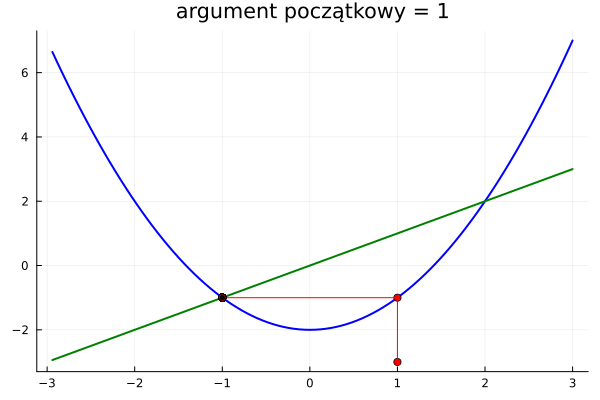
\includegraphics[scale=0.39]{plots/x^2-2:1.png}
    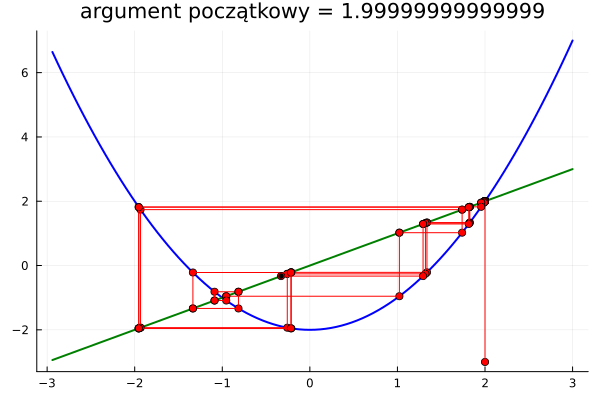
\includegraphics[scale=0.39]{plots/x^2-2:1.999.png}
    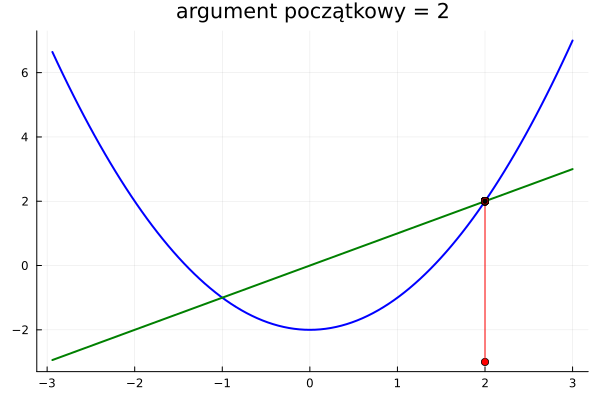
\includegraphics[scale=0.39]{plots/x^2-2:2.png}
    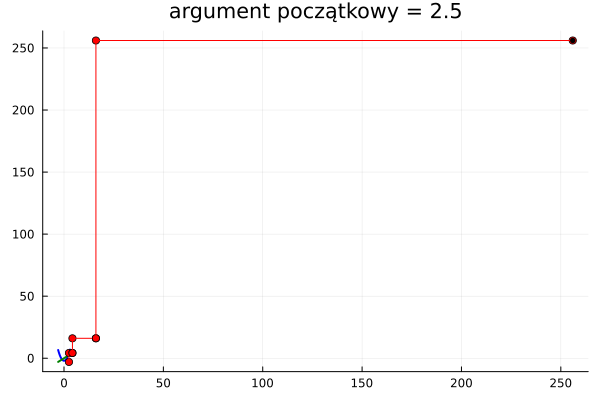
\includegraphics[scale=0.39]{plots/x^2-2:2.5.png}
    \caption{Iteracja graficzna dla $x_{n+1} = x_n^2 - 2$}
\end{figure}

\begin{figure}[h!]
    \centering
    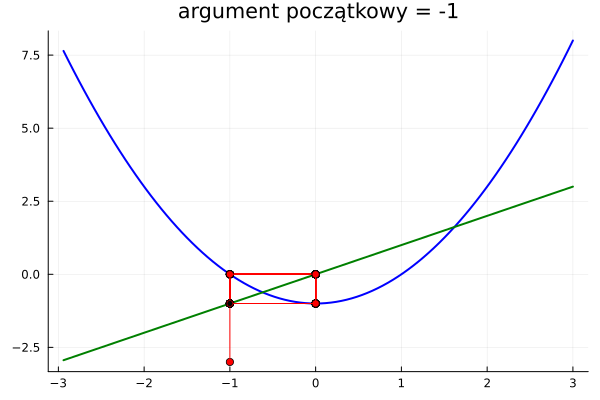
\includegraphics[scale=0.39]{plots/x^2-1:-1.png}
    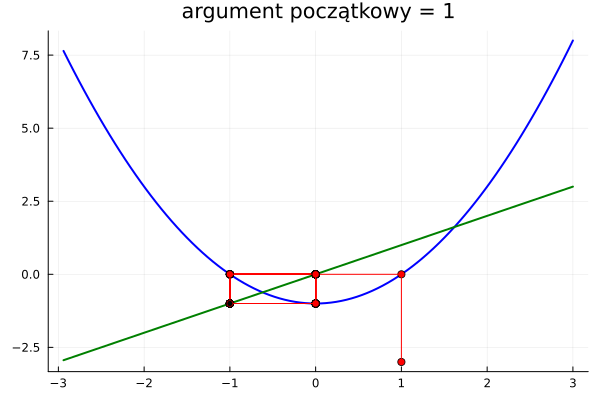
\includegraphics[scale=0.39]{plots/x^2-1:1.png}
    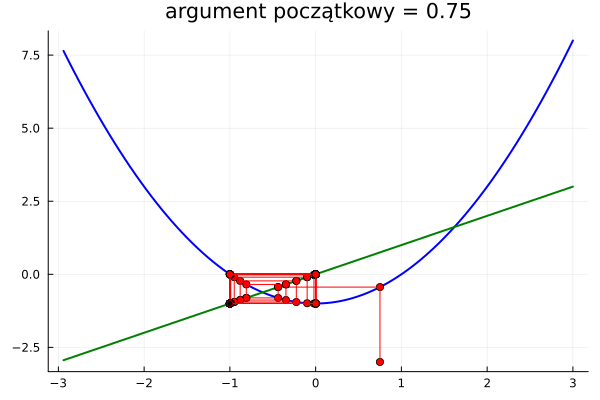
\includegraphics[scale=0.39]{plots/x^2-1:0.75.png}
    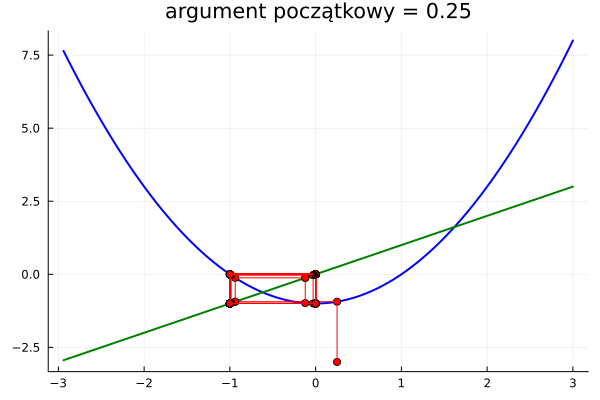
\includegraphics[scale=0.39]{plots/x^2-1:0.25.png}
    %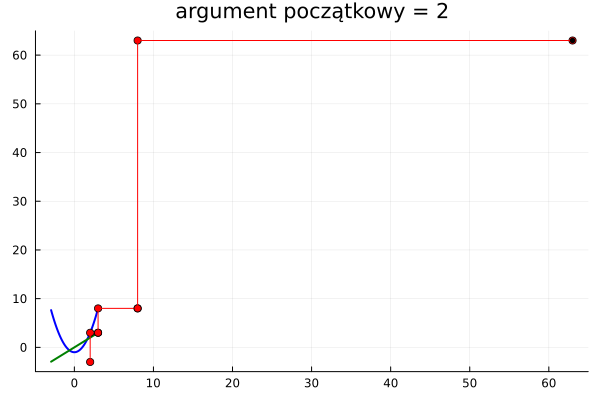
\includegraphics[scale=0.39]{plots/x^2-1:2.png}
    \caption{Iteracja graficzna dla $x_{n+1} = x_n^2 - 1$}
\end{figure}

\begin{table}[h!]
    \centering
    \begin{tabular}{ |c|c|c|c| }
    \hline
    $n$ & $x_n$ dla $x_0 = 1$ & $x_n$ dla $x_0 = 2$ & $x_n$ dla $x_0 = 1.99999999999999$  \\
    \hline
    1 & -1.0 & 2.0 & 1.99999999999996 \\
    \hline
    2 & -1.0 & 2.0 & 1.9999999999998401 \\
    \hline
    3 & -1.0 & 2.0 & 1.9999999999993605 \\
    \hline
    4 & -1.0 & 2.0 & 1.999999999997442 \\
    \hline
    5 & -1.0 & 2.0 & 1.9999999999897682 \\
    \hline
    6 & -1.0 & 2.0 & 1.9999999999590727 \\
    \hline
    7 & -1.0 & 2.0 & 1.999999999836291 \\
    \hline
    8 & -1.0 & 2.0 & 1.9999999993451638 \\
    \hline
    9 & -1.0 & 2.0 & 1.9999999973806553 \\
    \hline
    10 & -1.0 & 2.0 & 1.999999989522621 \\
    \hline
    11 & -1.0 & 2.0 & 1.9999999580904841 \\
    \hline
    12 & -1.0 & 2.0 & 1.9999998323619383 \\
    \hline
    13 & -1.0 & 2.0 & 1.9999993294477814 \\
    \hline
    14 & -1.0 & 2.0 & 1.9999973177915749 \\
    \hline
    15 & -1.0 & 2.0 & 1.9999892711734937 \\
    \hline
    16 & -1.0 & 2.0 & 1.9999570848090826 \\
    \hline
    17 & -1.0 & 2.0 & 1.999828341078044 \\
    \hline
    18 & -1.0 & 2.0 & 1.9993133937789613 \\
    \hline
    19 & -1.0 & 2.0 & 1.9972540465439481 \\
    \hline
    20 & -1.0 & 2.0 & 1.9890237264361752 \\
    \hline
    21 & -1.0 & 2.0 & 1.9562153843260486 \\
    \hline
    22 & -1.0 & 2.0 & 1.82677862987391 \\
    \hline
    23 & -1.0 & 2.0 & 1.3371201625639997 \\
    \hline
    24 & -1.0 & 2.0 & -0.21210967086482313 \\
    \hline
    25 & -1.0 & 2.0 & -1.9550094875256163 \\
    \hline
    26 & -1.0 & 2.0 & 1.822062096315173 \\
    \hline
    27 & -1.0 & 2.0 & 1.319910282828443 \\
    \hline
    28 & -1.0 & 2.0 & -0.2578368452837396 \\
    \hline
    29 & -1.0 & 2.0 & -1.9335201612141288 \\
    \hline
    30 & -1.0 & 2.0 & 1.7385002138215109 \\
    \hline
    31 & -1.0 & 2.0 & 1.0223829934574389 \\
    \hline
    32 & -1.0 & 2.0 & -0.9547330146890065 \\
    \hline
    33 & -1.0 & 2.0 & -1.0884848706628412 \\
    \hline
    34 & -1.0 & 2.0 & -0.8152006863380978 \\
    \hline
    35 & -1.0 & 2.0 & -1.3354478409938944 \\
    \hline
    36 & -1.0 & 2.0 & -0.21657906398474625 \\
    \hline
    37 & -1.0 & 2.0 & -1.953093509043491 \\
    \hline
    38 & -1.0 & 2.0 & 1.8145742550678174 \\
    \hline
    39 & -1.0 & 2.0 & 1.2926797271549244 \\
    \hline
    40 & -1.0 & 2.0 & -0.3289791230026702 \\
    \hline
    \end{tabular}
    \caption{Kolejne elementy ciągu opisanego równaniem $x_{n+1} = x_n^2 - 2$}
\end{table}

\begin{table}[h!]
    \centering
    \begin{tabular}{ |c|c|c|c|c| }
    \hline
    $n$ & $x_n$ dla $x_0 = 1$ & $x_n$ dla $x_0 = -1$ & $x_n$ dla $x_0 = 0.75$ & $x_n$ dla $x_0 = 0.25$ \\
    \hline
    1 & 0.0 & 0.0 & -0.4375 & -0.9375 \\
    \hline
    2 & -1.0 & -1.0 & -0.80859375 & -0.12109375 \\
    \hline
    3 & 0.0 & 0.0 & -0.3461761474609375 & -0.9853363037109375 \\
    \hline
    4 & -1.0 & -1.0 & -0.8801620749291033 & -0.029112368589267135 \\
    \hline
    5 & 0.0 & 0.0 & -0.2253147218564956 & -0.9991524699951226 \\
    \hline
    6 & -1.0 & -1.0 & -0.9492332761147301 & -0.0016943417026455965 \\
    \hline
    7 & 0.0 & 0.0 & -0.0989561875164966 & -0.9999971292061947 \\
    \hline
    8 & -1.0 & -1.0 & -0.9902076729521999 & -5.741579369278327e-6 \\
    \hline
    9 & 0.0 & 0.0 & -0.01948876442658909 & -0.9999999999670343 \\
    \hline
    10 & -1.0 & -1.0 & -0.999620188061125 & -6.593148249578462e-11 \\
    \hline
    11 & 0.0 & 0.0 & -0.0007594796206411569 & -1.0 \\
    \hline
    12 & -1.0 & -1.0 & -0.9999994231907058 & 0.0 \\
    \hline
    13 & 0.0 & 0.0 & -1.1536182557003727e-6 & -1.0 \\
    \hline
    14 & -1.0 & -1.0 & -0.9999999999986692 & 0.0 \\
    \hline
    15 & 0.0 & 0.0 & -2.6616486792363503e-12 & -1.0 \\
    \hline
    16 & -1.0 & -1.0 & -1.0 & 0.0 \\
    \hline
    17 & 0.0 & 0.0 & 0.0 & -1.0 \\
    \hline
    18 & -1.0 & -1.0 & -1.0 & 0.0 \\
    \hline
    19 & 0.0 & 0.0 & 0.0 & -1.0 \\
    \hline
    20 & -1.0 & -1.0 & -1.0 & 0.0 \\
    \hline
    21 & 0.0 & 0.0 & 0.0 & -1.0 \\
    \hline
    22 & -1.0 & -1.0 & -1.0 & 0.0 \\
    \hline
    23 & 0.0 & 0.0 & 0.0 & -1.0 \\
    \hline
    24 & -1.0 & -1.0 & -1.0 & 0.0 \\
    \hline
    25 & 0.0 & 0.0 & 0.0 & -1.0 \\
    \hline
    26 & -1.0 & -1.0 & -1.0 & 0.0 \\
    \hline
    27 & 0.0 & 0.0 & 0.0 & -1.0 \\
    \hline
    28 & -1.0 & -1.0 & -1.0 & 0.0 \\
    \hline
    29 & 0.0 & 0.0 & 0.0 & -1.0 \\
    \hline
    30 & -1.0 & -1.0 & -1.0 & 0.0 \\
    \hline
    31 & 0.0 & 0.0 & 0.0 & -1.0 \\
    \hline
    32 & -1.0 & -1.0 & -1.0 & 0.0 \\
    \hline
    33 & 0.0 & 0.0 & 0.0 & -1.0 \\
    \hline
    34 & -1.0 & -1.0 & -1.0 & 0.0 \\
    \hline
    35 & 0.0 & 0.0 & 0.0 & -1.0 \\
    \hline
    36 & -1.0 & -1.0 & -1.0 & 0.0 \\
    \hline
    37 & 0.0 & 0.0 & 0.0 & -1.0 \\
    \hline
    38 & -1.0 & -1.0 & -1.0 & 0.0 \\
    \hline
    39 & 0.0 & 0.0 & 0.0 & -1.0 \\
    \hline
    40 & -1.0 & -1.0 & -1.0 & 0.0 \\
    \hline
    \end{tabular}
    \caption{Kolejne elementy ciągu opisanego równaniem $x_{n+1} = x_n^2 - 1$}
\end{table}

\end{document}